\documentclass{article}

\usepackage{graphicx}
\usepackage{tikz}
\usepackage{tikzsymbols}
\usetikzlibrary{calc,patterns,shapes.geometric}
\pagestyle{empty}
\usepackage[margin=0pt]{geometry}
\geometry{papersize={14in,12in}}

\def\centerarc[#1](#2)(#3:#4:#5){\draw[#1] ($(#2)+({#5*cos(#3)},{#5*sin(#3)})$) arc (#3:#4:#5);}

\begin{document}
	\begin{figure}
		\centering
		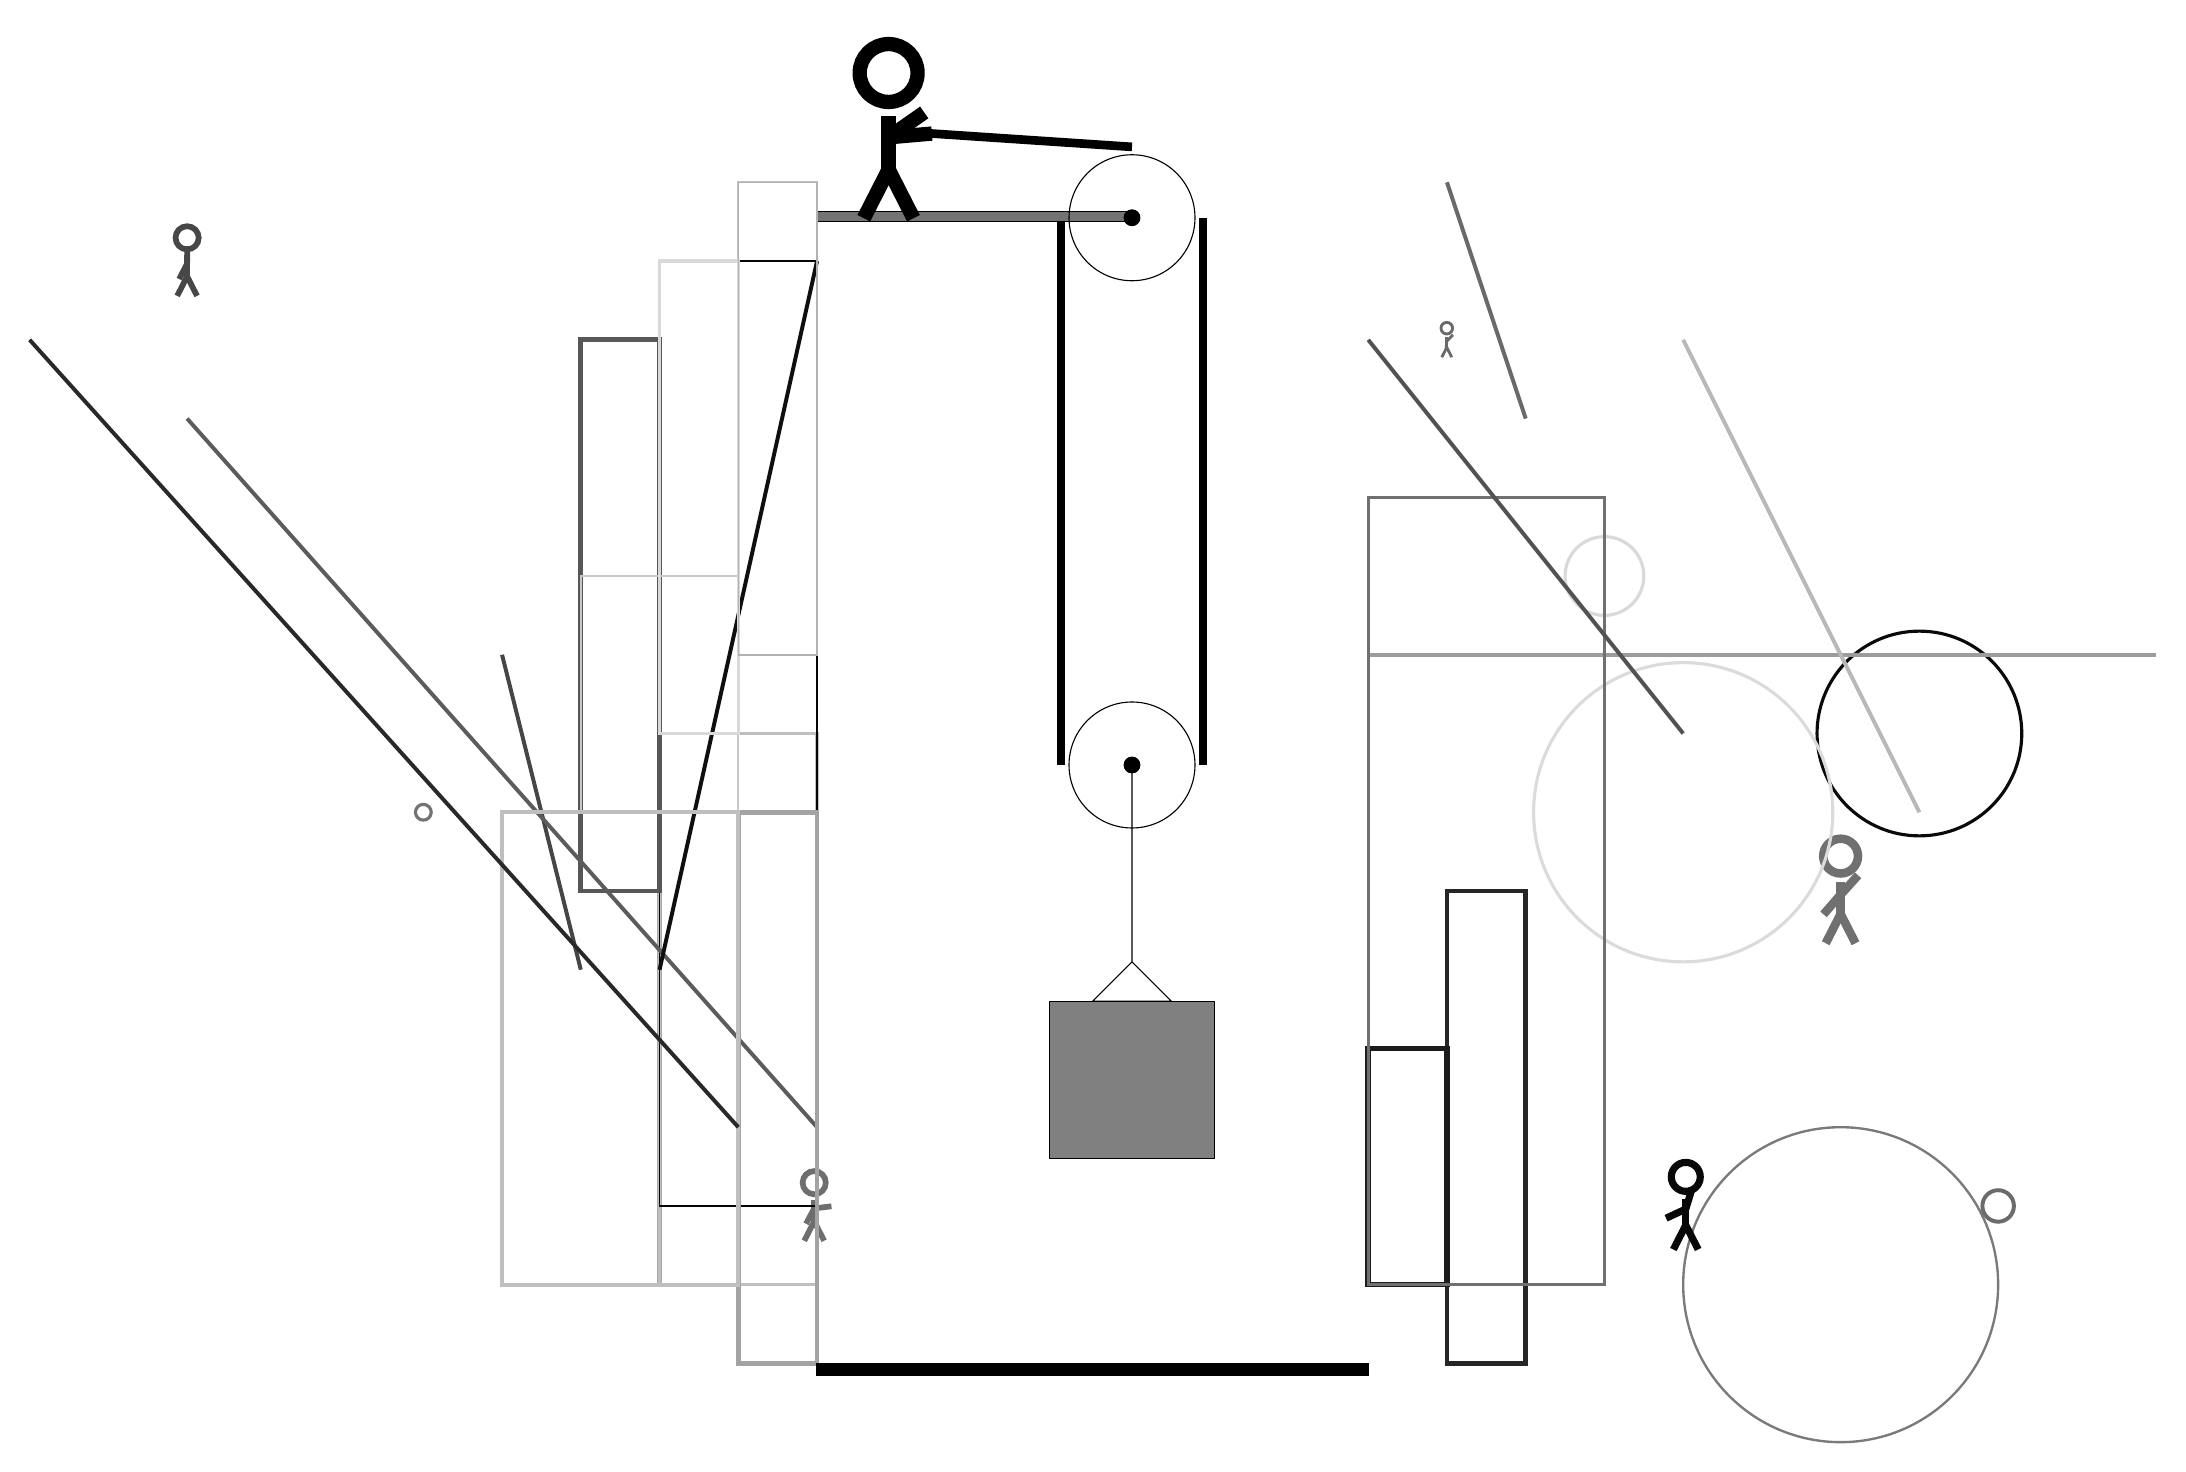
\begin{tikzpicture}
			%%%%% START %%%%%
			
			\draw[fill=black!55] (-2, 11.5) rectangle (2, 11.625);
			
			\draw (2, 4.6) circle (0.8);
			\draw[fill=black] (2, 4.6) circle (0.1);
			
			\draw (2, 11.55) circle (0.8);
			\draw[fill=black] (2, 11.55) circle (0.1);
			
			\draw (2, 4.6) -- (2, 2.1) -- (1.5, 1.6) -- (2.5, 1.6) -- (2, 2.1);
			\draw[fill=black!50] (0.95, 1.6) rectangle (3.05, -0.4);
			
			\draw [line width=0.4mm, color=black!96](12, 5) circle (1.3);
			
			\draw[line width=0.6mm, color=black!34] (-4, -2) rectangle (-4, 8);
			\draw[line width=0.3mm, color=black!25] (-3, -2) rectangle (-2, 12);
			\draw[line width=0.5mm, color=black!59](6, 12) -- (7, 9);
			\node[line width=0.2mm, color=black!57] at (-2, -1) {\Strichmaxerl[4][62][7]};
			\draw[line width=0.4mm, color=black!25] (-2, 5) rectangle (-4, -2);
			\draw[line width=0.2mm, color=black!98] (-4, -1) rectangle (-2, 11);
			\draw[line width=0.3mm, color=black!93] (-3, -1) rectangle (-3, 7);
			\draw[line width=0.6mm, color=black!85] (7, 3) rectangle (6, -3);
			\draw[line width=0.5mm, color=black!73](-6, 6) -- (-5, 2);
			
			\node[line width=0.2mm, color=black!56] at (11, 3) {\Strichmaxerl[6][49][48]};
			\node[line width=0.6mm, color=black!59] at (6, 10) {\Strichmaxerl[2][85][45]};
			\draw[line width=0.6mm, color=black!66] (-4, 3) rectangle (-5, 10);
			
			\draw[line width=0.5mm, color=black!39](5, 6) -- (15, 6);
			\draw [line width=0.3mm, color=black!52](11, -2) circle (2.0);
			\draw[line width=0.5mm, color=black!64](-2, 0) -- (-10, 9);
			
			\draw[line width=0.5mm, color=black!94](-4, 2) -- (-2, 11);
			\draw[line width=0.7mm, color=black!89] (5, 1) rectangle (6, -2);
			\draw [line width=0.4mm, color=black!15](8, 7) circle (0.5);
			\node[line width=0.2mm, color=black!97] at (9, -1) {\Strichmaxerl[5][25][73]};
			\node[line width=0.7mm, color=black!72] at (-10, 11) {\Strichmaxerl[4][63][89]};
			
			\draw [line width=0.4mm, color=black!55](-7, 4) circle (0.1);
			
			\draw[line width=0.6mm, color=black!36] (-3, 4) rectangle (-2, -3);
			\draw [line width=0.4mm, color=black!14](9, 4) circle (1.9);
			\draw[line width=0.4mm, color=black!56] (5, -2) rectangle (8, 8);
			\draw[line width=0.3mm, color=black!22] (-3, 7) rectangle (-5, 4);
			
			\draw[line width=0.5mm, color=black!28](9, 10) -- (12, 4);
			\draw[line width=0.5mm, color=black!68](9, 5) -- (5, 10);
			\draw[line width=0.5mm, color=black!25] (-3, 4) rectangle (-6, -2);
			\draw [line width=0.5mm, color=black!58](13, -1) circle (0.2);
			\draw[line width=0.5mm, color=black!84](-3, 0) -- (-12, 10);
			\draw[line width=0.4mm, color=black!15] (-3, 11) rectangle (-4, 5);
			\draw[line width=0.2mm, color=black!30] (-2, 12) rectangle (-3, 6);
			
			\draw[line width=1.1mm] (1.1, 11.5) -- (1.1, 4.6);
			\centerarc[line width=1.1mm](2, 4.6)(180:360:0.9);
			\draw[line width=1.1mm](2.9, 4.6) -- (2.9, 11.55);
			\centerarc[line width=1.1mm](2, 11.55)(0:90:0.9);
			\draw[line width=1.1mm](2, 12.45) -- (-1, 12.65);
			
			\node at (-1, 12.65) {\Strichmaxerl[10][-175][35]};
			
			\draw[fill=black] (-2, -3) rectangle (5, -3.15);
			
			%%%%% END %%%%%
		\end{tikzpicture}
	\end{figure}	
\end{document}